\documentclass{beamer}

\usepackage{iftex}
\ifPDFTeX
  \usepackage[T1]{fontenc}
  \PackageWarningNoLine{NTU Beamer}{Use XeLaTeX or LuaLaTeX for Chinese text}
\else
  % scheme=plain keeps English document labels while enabling CJK text.
  \usepackage[UTF8,scheme=plain]{ctex}
\fi

\usepackage{hyperref}
\usepackage{latexsym,amsmath,xcolor,multicol,booktabs,calligra}
\usepackage{graphicx,pstricks,listings,stackengine}

\author{Author Name}
\title{NTU Beamer Theme}
\subtitle{Unofficial Classic Presentation Template}
\institute{Nanyang Technological University}
\date{\today}
\usepackage{NTU}

% Helpers used by the command-reference slides.
\def\cmd#1{\texttt{\color{ntubrightblue}\footnotesize $\backslash$#1}}
\def\env#1{\texttt{\color{blue}\footnotesize #1}}
\definecolor{deepblue}{rgb}{0,0,0.5}
\definecolor{deepnavy}{RGB}{24,28,98}
\definecolor{deepgreen}{rgb}{0,0.5,0}
\definecolor{halfgray}{gray}{0.55}

\lstset{
  basicstyle=\ttfamily\small,
  keywordstyle=\bfseries\color{deepblue},
  emphstyle=\ttfamily\color{deepnavy},
  stringstyle=\color{deepgreen},
  numbers=left,
  numberstyle=\small\color{halfgray},
  rulesepcolor=\color{ntubrightblue!20!green!20!blue!20},
  frame=shadowbox,
}

\begin{document}

\begin{frame}
  \titlepage
  \begin{figure}
    \centering
    
\includegraphics[width=0.35\linewidth]{pic/NTU_Logo.png}
  \end{figure}
\end{frame}

\begin{frame}{Contents}
  \tableofcontents[
    sectionstyle=show,
    subsectionstyle=show/shaded/hide,
    subsubsectionstyle=show/shaded/hide
  ]
\end{frame}

\section{Getting Started}

\begin{frame}{Why Use Beamer?}
  \begin{itemize}[<+-| alert@+>]
    \item This is an unofficial community template and is not endorsed by NTU.
    \item Beamer provides consistent, reproducible presentation layouts.
    \item The same \LaTeX{} tools can be used for papers, equations, and slides.
    \item This template applies NTU Blue to the title bars, navigation, and footer.
    \item The supplied logo is loaded from \texttt{pic/NTU\_Logo.png}.
    \item Compile with Xe\LaTeX{} or Lua\LaTeX{} when the deck contains Chinese text.
  \end{itemize}
\end{frame}

\subsection{Multilingual Support}

\begin{frame}{English and Chinese}
  English is the default presentation language. The template also loads
  \texttt{ctex} when compiled with Xe\LaTeX{} or Lua\LaTeX{}, so Chinese can
  be used wherever it is needed.

  \begin{block}{Chinese example}
    \kaishu
    南洋理工大学欢迎您。这个模板支持中英文混合排版。
  \end{block}

  \begin{exampleblock}{Source}
    \texttt{\textbackslash kaishu} may be applied locally to Chinese text;
    it is no longer applied to the entire English presentation.
  \end{exampleblock}
\end{frame}

\section{Theme Design}

\subsection{NTU Branding}

\begin{frame}{Theme Features}
  \begin{itemize}
    \item A compact navigation bar keeps section markers on one line.
    \item NTU Blue is the primary color throughout the presentation.
    \item The footer displays the author, institution, title, and frame count.
    \item Numbered captions and text-style bibliography entries are enabled.
    \item The theme remains easy to extend for courses, conferences, and research groups.
    \item The sample bibliography retains a reference to the original theme \cite{origin}.
  \end{itemize}
\end{frame}

\subsection{Why \LaTeX?}

\begin{frame}{Document Preparation}
  \begin{table}
    \centering
    \small
    \begin{tabular}{p{0.43\linewidth}|p{0.43\linewidth}}
      \textbf{Word processor} & \textbf{\LaTeX} \\
      \hline
      Direct visual editing & Content-driven typesetting \\
      Manual formatting is common & Styles remain consistent \\
      Long documents require careful maintenance & Long and short documents use the same workflow \\
      Equation tools vary by application & Mathematical typesetting is a core strength \\
      Usually stored in a binary format & Source files are readable plain text \\
      Often requires a commercial licence & Free and open-source tooling is available \\
    \end{tabular}
  \end{table}
\end{frame}

\section{Beamer Examples}

\subsection{Typesetting}

\begin{frame}[fragile]{Equation Layout}
  \begin{exampleblock}{Unnumbered equation}
    \begin{equation*}
      J(\theta)
      = \mathbb{E}_{\pi_\theta}[G_t]
      = \sum_{s\in\mathcal{S}} d^\pi(s)
        \sum_{a\in\mathcal{A}}\pi_\theta(a|s)Q^\pi(s,a)
    \end{equation*}
  \end{exampleblock}

  \begin{exampleblock}{Aligned equations}
    Use \verb|\mathrm{}| or \verb|\text{}| for words inside mathematics.
    \begin{align}
      Q_\mathrm{target}
        &= r+\gamma Q^\pi(s^\prime,\pi_\theta(s^\prime)+\epsilon),\\
      \epsilon
        &\sim\mathrm{clip}(\mathcal{N}(0,\sigma),-c,c).\nonumber
    \end{align}
  \end{exampleblock}
\end{frame}

\begin{frame}{Numbered Multiline Equation}
  \begin{exampleblock}{Multline environment}
    \begin{multline}
      A=\lim_{n\rightarrow\infty}\Delta x
      \left(a^{2}
      +\left(a^{2}+2a\Delta x+\left(\Delta x\right)^{2}\right)\right.\\
      +\left(a^{2}+2\cdot2a\Delta x+2^{2}\left(\Delta x\right)^{2}\right)
      +\ldots\\
      \left.
      +\left(a^{2}+2\cdot(n-1)a\Delta x
      +(n-1)^{2}\left(\Delta x\right)^{2}\right)\right)\\
      =\frac{1}{3}\left(b^{3}-a^{3}\right).
    \end{multline}
  \end{exampleblock}
\end{frame}

\begin{frame}{Graphics and Columns}
  \begin{minipage}[c]{0.3\linewidth}
    \psset{unit=0.55cm}
    \begin{pspicture}(-1.75,-3)(3.25,4)
      \psline[linewidth=0.25pt](0,0)(0,4)
      \rput[tl]{0}(0.2,2){$\vec e_z$}
      \rput[tr]{0}(-0.9,1.4){$\vec e$}
      \rput[tl]{0}(2.8,-1.1){$\vec C_{\mathrm{ext}}$}
      \rput[br]{0}(-0.3,2.1){$\theta$}
      \rput{25}(0,0){%
        \psframe[fillstyle=solid,fillcolor=lightgray,linewidth=.8pt](-0.1,-3.2)(0.1,0)}
      \rput{25}(0,0){%
        \psellipse[fillstyle=solid,fillcolor=yellow,linewidth=3pt](0,0)(1.5,0.5)}
      \rput{25}(0,0){%
        \psframe[fillstyle=solid,fillcolor=lightgray,linewidth=.8pt](-0.1,0)(0.1,3.2)}
      \rput{25}(0,0){%
        \psline[linecolor=ntubrightblue,linewidth=1.5pt]{->}(0,0)(0,2)}
      \psline[linecolor=ntubrightblue,linewidth=1.25pt]{->}(0,0)(3,-1)
      \psarc{->}{2.1}{90}{112.5}
      \rput[bl](.1,.01){C}
    \end{pspicture}
  \end{minipage}\hspace{1cm}
  \begin{minipage}{0.5\linewidth}
    \begin{figure}
      \centering
      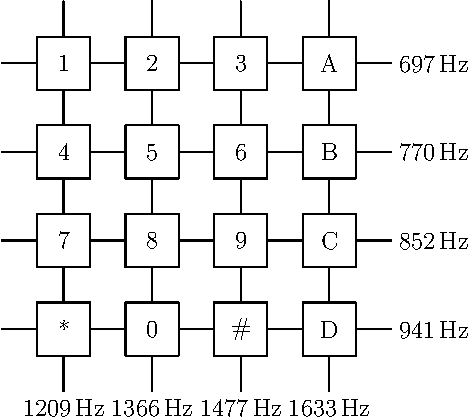
\includegraphics[height=.4\textheight]{pic/dtmf.pdf}
      \caption{A second figure in an adjacent column}
    \end{figure}
  \end{minipage}
\end{frame}

\subsection{Commands and Environments}

\begin{frame}[fragile]{Common \LaTeX{} Commands}
  \begin{exampleblock}{Commands}
    \centering
    \footnotesize
    \begin{tabular}{llll}
      \cmd{chapter} & \cmd{section} & \cmd{subsection} & \cmd{paragraph} \\
      Chapter & Section & Subsection & Titled paragraph \\\hline
      \cmd{centering} & \cmd{emph} & \cmd{verb} & \cmd{url} \\
      Centre & Emphasise & Verbatim text & Hyperlink \\\hline
      \cmd{footnote} & \cmd{item} & \cmd{caption} & \cmd{includegraphics} \\
      Footnote & List item & Caption & Insert image \\\hline
      \cmd{label} & \cmd{cite} & \cmd{ref} \\
      Label & Cite a source & Cross-reference \\\hline
    \end{tabular}
  \end{exampleblock}

  \begin{exampleblock}{Environments}
    \centering
    \footnotesize
    \begin{tabular}{lll}
      \env{table} & \env{figure} & \env{equation} \\
      Table & Figure & Equation \\\hline
      \env{itemize} & \env{enumerate} & \env{description} \\
      Bulleted list & Numbered list & Description list \\\hline
    \end{tabular}
  \end{exampleblock}
\end{frame}

\begin{frame}[fragile]{List Environments}
  \begin{minipage}{0.5\linewidth}
\begin{lstlisting}[language=TeX]
\begin{itemize}
  \item First item
  \item Second item
  \begin{itemize}
    \item Nested item
  \end{itemize}
\end{itemize}
\end{lstlisting}
  \end{minipage}\hspace{1cm}
  \begin{minipage}{0.3\linewidth}
    \begin{itemize}
      \item First item
      \item Second item
      \begin{itemize}
        \item Nested item
      \end{itemize}
    \end{itemize}
  \end{minipage}

  \medskip
  \pause

  \begin{minipage}{0.5\linewidth}
\begin{lstlisting}[language=TeX]
\begin{enumerate}
  \item Beginner
  \item Intermediate
  \item Advanced
\end{enumerate}
\end{lstlisting}
  \end{minipage}\hspace{1cm}
  \begin{minipage}{0.3\linewidth}
    \begin{enumerate}
      \item Beginner
      \item Intermediate
      \item Advanced
    \end{enumerate}
  \end{minipage}
\end{frame}

\begin{frame}[fragile]{Mathematical Expressions}
  \begin{columns}
    \begin{column}{.55\textwidth}
\begin{lstlisting}[language=TeX]
$V = \frac{4}{3}\pi r^3$

\[
  V = \frac{4}{3}\pi r^3
\]

\begin{equation}
  \label{eq:vsphere}
  V = \frac{4}{3}\pi r^3
\end{equation}
\end{lstlisting}
    \end{column}
    \begin{column}{.4\textwidth}
      Inline: $V = \frac{4}{3}\pi r^3$
      \[
        V = \frac{4}{3}\pi r^3
      \]
      \begin{equation}
        \label{eq:vsphere}
        V = \frac{4}{3}\pi r^3
      \end{equation}
    \end{column}
  \end{columns}
  \begin{itemize}
    \item See the
      \href{https://en.wikibooks.org/wiki/LaTeX/Mathematics}
      {\color{ntubrightblue}{\LaTeX{} mathematics guide}}
      for more examples.
  \end{itemize}
\end{frame}

\begin{frame}[fragile]{Tables and Cross-References}
  \begin{columns}
    \column{.57\textwidth}
\begin{lstlisting}[language=TeX]
\begin{table}
  \caption{Number and value}
  \label{tab:number}
  \begin{tabular}{cl}
    \toprule
    Number & Value \\
    \midrule
    1 & 4.0 \\
    2 & 3.7 \\
    \bottomrule
  \end{tabular}
\end{table}
See Equation~\ref{eq:vsphere}
and Table~\ref{tab:number}.
\end{lstlisting}
    \column{.38\textwidth}
      \begin{table}
        \centering
        \caption{Number and value}
        \label{tab:number}
        \begin{tabular}{cl}
          \toprule
          Number & Value \\\midrule
          1 & 4.0\\
          2 & 3.7\\\bottomrule
        \end{tabular}
      \end{table}
      See Equation~(\ref{eq:vsphere}) and Table~\ref{tab:number}.
  \end{columns}
\end{frame}

\begin{frame}{Choosing Graphic Formats}
  \begin{itemize}
    \item Prefer vector graphics such as PDF, EPS, and PS for diagrams.
    \begin{itemize}
      \item Useful tools include PGF/TikZ, PSTricks, Inkscape, and Visio.
      \item Charts from MATLAB or Excel can be exported as PDF.
    \end{itemize}
    \item Use raster graphics such as PNG, JPEG, and TIFF for photographs.
    \begin{itemize}
      \item Export at sufficient resolution to avoid visible blur.
      \item Avoid raster formats for line art when a vector source is available.
    \end{itemize}
  \end{itemize}
  \begin{figure}
    \centering
    
\includegraphics[width=0.28\linewidth]{pic/NTU_Logo.png}
    \caption{NTU logo example}
  \end{figure}
\end{frame}

\section{Example Schedule}

\begin{frame}{Project Timeline}
  \begin{itemize}
    \item January: complete the literature review.
    \item February: evaluate candidate presentation structures.
    \item March and April: develop and test the NTU Beamer theme.
    \item May: prepare the final report and presentation.
  \end{itemize}
\end{frame}

\section{References}

\begin{frame}[allowframebreaks]{References}
  \bibliography{ref}
  \bibliographystyle{alpha}
  % Use \tiny before \bibliography if the reference list is unusually long.
\end{frame}

\begin{frame}
  \begin{center}
    {\Huge\calligra Thank you!}
  \end{center}
\end{frame}

\end{document}
